\section{Method}
\label{section:method}
%In this section, the method used to find an answer to the research questions should be presented. 

%If this report presents results from a literature search, this means providing sufficient information 
%for allowing someone else to repeat the literature search and compare the results. I.e., a search using 
%the phrases a, b, and c, was made in database x, y and z on the date Month Date, Year (e.g., July 31st, 
%2021). The search resulted in x hits. Then, information on how you chose which works to include in this 
%report should be provided. The references should be used for answering your research questions.

%If the work reports on an experiment, this part should provide information about the experimental setup, 
%how the experiment was conducted, how data was collected and analyzed etc. Motivate methodological choices 
%through references. Also an experiment should be presented with sufficient detail such that it can be 
%repeated by someone else.

\subsection{Signal Aqusition}
A setup consisting of a Digilent Analog Discovery studio measurement device, two Myoware muscle sensor 
kits, various weights from none to weights of up to six kilograms and a resistance 
band were used during the signal acquisition. The Myoware sensors are connected to the Analog Discovery 
oscilloscopes, ground and a 3.3 voltage input. Two oscilloscopes are connected to the two Myoware 
sensors, one for the bicep and one for the tricep. The bicep sensor was placed with one end in the 
middle of the biceps brachii while tensed, the other end was placed along the grain of the muscle 
towards the elbow, and the reference was placed between the bicep and triceps on the inside of the arm. 
The triceps sensor was placed with one end in the middle of the long head of the triceps brachii while 
tensed, the other end was placed along the grain of the muscle towards the elbow, and the reference was 
placed either between the bicep and triceps on the inner arm or on the elbow depending on the which would 
be more easily reached. Measurement data is acquired using the Digilent Waveforms program. In Waveforms a 
script was created with javascript code where data is labeled from 0-3 with each state representing a 
different action, 0 = static down, 1 = moving up, 2 = static up, 3 = moving down. Two LED lights show what 
movement is expected from the user and the data is collected and labeled accordingly. Which test subject, 
which arm, what weight was used and what direction the weight was providing resistance in were all recorded.


\subsection{\acrfull{rnn}}
With the objective of having a reliable method for \acrshort{emg} based continuous motion prediction, we chose to 
use a \acrshort{rnn} as our AI model. Since the purpose of the project is to end with a working exoskeleton based 
on the RoboRIO system, an embedded solution had to be found. This resulted in two different \acrshort{rnn} 
implementations for the same model:
\begin{itemize}

    \item \textbf{Python implementation:} The first implementation was done using Python and the PyTorch library. 
    This implementation was used to train the model, test its accuracy and extract its parameters.
    
    \item \textbf{LabView implementation:} The second implementation was done using LabView and the RoboRIO system. 
    This implementation was used to import the Python parameters to use the \acrshort{rnn} in a real-time scenario.

\end{itemize}

Before going through with implementing the model, a design was made. The final model is based on the work of \cite{RNNEMG} 
as their \acrfull{lstm} implementation provided promising results both in accuracy and inference time. The model consists 
of four layers:
\begin{itemize}

    \item Input layer

    \item First \acrshort{lstm} layer

    \item Second \acrshort{lstm} layer
    
    \item Output layer

\end{itemize}

\cite{RNNEMG} proposed different ranges of values for parameters such as the number of nodes in each one of the \acrshort{lstm} 
layers, the learning rate, and the number of epochs in the training process, which were then optimized by a \acrfull{gwo} 
algorithm for their specific dataset. However, due to hardware restrictions, running such an optimizer was not possible. Instead, 
the parameters were chosen by trial and error, CHANGE a process during which we realized that the model provided a perfect accuracy 
for our dataset leading to the conclusion that the number of epochs could be reduced to 1 and the final model would be chosen 
by the one that provided the lowest inference time CHANGE. Figure \ref{fig:rnn_struct} shows the structure of our final model after 
the selection process and table \ref{table:rnn_params} shows the parameters used.

\begin{figure}[h]
    \centering
    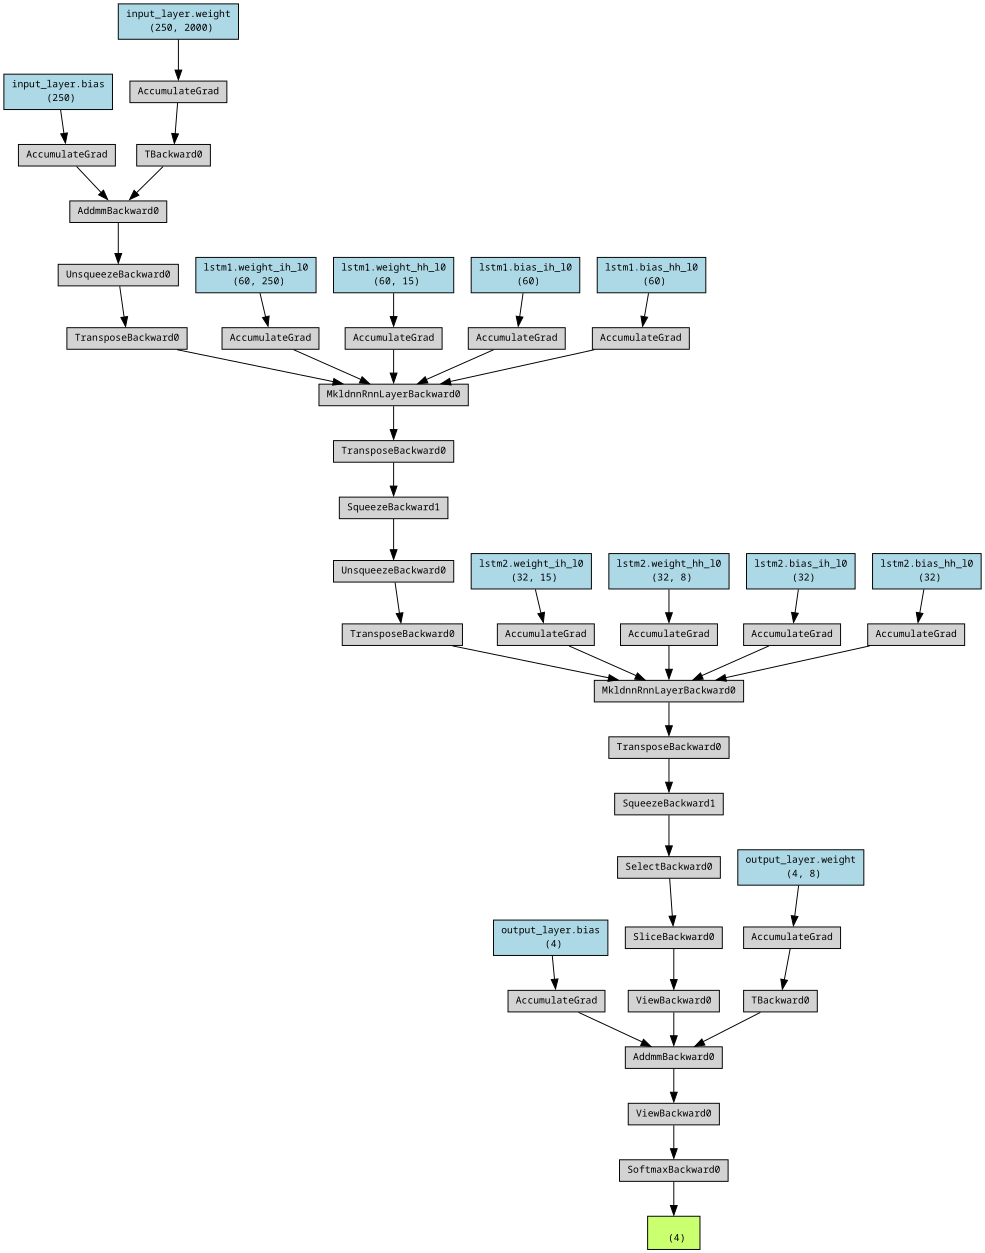
\includegraphics[scale=0.25]{images/rnn_struct.png}
    \caption{Structure of the final \acrshort{rnn} model}
    \label{fig:rnn_struct}
\end{figure}

\begin{table}[h]
    \centering
    \begin{tabular}{|c|c|}
    \hline
    \textbf{Parameter} & \textbf{Value} \\ \hline
    Number of nodes in the input layer & 250 \\ \hline
    Number of nodes in the first \acrshort{lstm} layer & 15 \\ \hline
    Number of nodes in the second \acrshort{lstm} layer & 8 \\ \hline
    Number of output classes & 4 \\ \hline
    Learning rate & 0.00502 \\ \hline
    Number of epochs & CHANGE \\ \hline
    \end{tabular}
    \caption{Parameters of the \acrshort{rnn} model}
    \label{table:rnn_params}
\end{table}

\subsection{Python Implementation}
The Python implementation of the \acrshort{rnn} was done using the PyTorch library as it provided facilities 
to create and train the model while using LSTM layers. The model runs once over the training set, then it is 
tested over the test set where the accuracy and average inference time are calculated. After the model is trained 
and tested, it is saved both in a .pth file and a .xml file to be used in LabView.
Originally, a script using the \acrshort{gwo} algorithm was implemented 
to optimize the parameters of the model, however, due to the limitations mentioned before, this script was not 
used and instead, a different script with a manual parameter selection was used.

\subsubsection{Data preprocessing}
The collected data was preprocessed before being fed into the model. Firstly, the data files were mixed in order to 
avoid having the model learn patterns based on the state of the muscles of the test subject or on the test subject itself.

\subsection{Labview}

\subsection{Labview Implementation}
The LabView implementation was multifacated, with three destinct parts. The first being the preprocessing, done on a separate machine to process the .xml files into properly set up .bin files able
to be read by the embedded system. The second being data acquisition done on the \acrfull(FPGA) which opens two ports and reads the voltage continuously. The third one being the Real Time system which
initialises all connections, and loads settings and weights. It then runs a loop of data gathering from the \acrshort(FPGA) then running it through the RNN which output is interpretated into a single 
value to be sent through the CAN buss to a motor controller. If the loop is interupted it follows a termination of all the connections.